\begin{alertblock}{The Sliding Window Approach}
	\begin{itemize}
		\item Window Size $w$
		\item Stride $s$	
	\end{itemize}
	\centering
	\only<1>{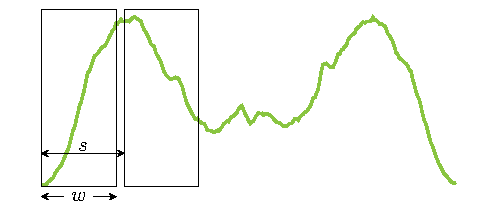
\includegraphics[width=0.8\textwidth]{figures/sliding_window.pdf} \\}
	\only<2>{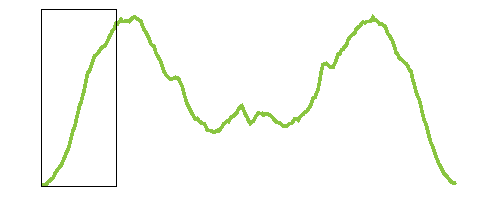
\includegraphics[width=0.8\textwidth]{figures/sliding_window_0.pdf} \\}
	\only<3>{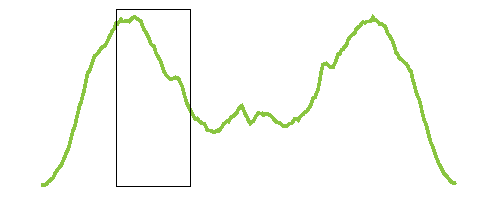
\includegraphics[width=0.8\textwidth]{figures/sliding_window_1.pdf} \\}
	\only<4>{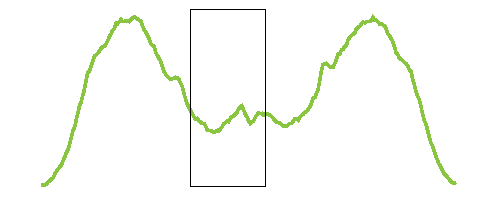
\includegraphics[width=0.8\textwidth]{figures/sliding_window_2.pdf} \\}
	\only<5>{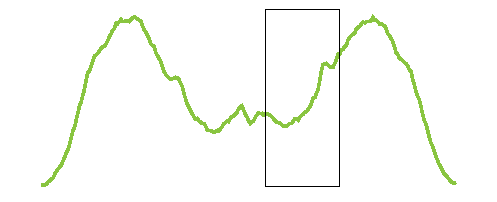
\includegraphics[width=0.8\textwidth]{figures/sliding_window_3.pdf} \\}
	\only<6>{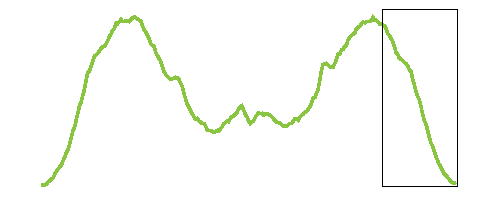
\includegraphics[width=0.8\textwidth]{figures/sliding_window_4.pdf} \\}
	\vspace*{0.5cm}
	\begin{tikzpicture}
	
		\only<2-6>\draw [decorate, decoration={brace, amplitude=5pt, raise=2pt, mirror}] (-2.5,-1.5) -- (6.0,-1.5) node [below, midway, yshift=-2mm] {Subsequence Collection};
		
	
		\only<2-6>{\node[inner sep=0pt] (ts) at (-2,-1)
		{
\includegraphics[height=1.2cm]{figures/subsequences_for_SW_0.pdf}};}
		
		\only<3-6>{\node[inner sep=0pt] (ts) at (-0.5,-1)
		{
\includegraphics[height=1.2cm]{figures/subsequences_for_SW_1.pdf}};}
		
		\only<4-6>{\node[inner sep=0pt] (ts) at (1.5,-1)
		{
\includegraphics[height=1.2cm]{figures/subsequences_for_SW_2.pdf}};}
		
		\only<5-6>{\node[inner sep=0pt] (ts) at (3.5,-1)
		{
\includegraphics[height=1.2cm]{figures/subsequences_for_SW_3.pdf}};}
		
		\only<6>{\node[inner sep=0pt] (ts) at (5.5,-1)
		{
\includegraphics[height=1.2cm]{figures/subsequences_for_SW_4.pdf}};}

	\end{tikzpicture}
\end{alertblock}